Task 1 includes downloading the Vadere \cite{vadere} software, e.g. downloading the compiled JAR files from the official website. They can be run by navigating to the location where the files are saved via the command window. Then, the following line must be run in order to open the Graphical User Interface: \texttt{java -jar vadere-gui.jar}

In this task, we will take a look at three scenarios that were already highlighted in our automaton from exercise sheet 1. In Vadere, the Optimal Steps Model is used to run the scenarios. "The Optimal Steps Model (OSM) is a pedestrian locomotion model that operationalizes an individual’s need for personal space." \cite{mayr2022social} \\ 

% OSM: 
% - RiMEA 1
% - RiMEA 6
% - Chicken Test
% --> observations
% --> differences to automaton

\textbf{RiMEA scenario 1 (straight line):}\\
Parameters of simulation 1
\begin{itemize}
    \item height and width of the pedestrian: 0.4m 
    \item corridor: 40m long 
\end{itemize}

The Vadere software offers a larger variation of features than our automaton from exercise 1. The following tabs are available in the application: 

\begin{itemize}
    \item Simulation: settings e.g. for time can be found
    \item Model: where different templates can be loaded
    \item Psychology: not used for this exercise
    \item Topography: JSON structure of the current scenario
    \item Stimuli: not used for this exercise
    \item Data output: determine which files will be created when running a scenario
    \item Topography creator: GUI with different buttons to create your own scenario
\end{itemize}

After running a scenario, a new tab appears, called 'Post-Visualization'. It is useful to check upon any arbitrary time step of the simulation.

\begin{figure}[H]
 \centering
 \begin{subfigure}[b]{0.4\textwidth}
     \centering
     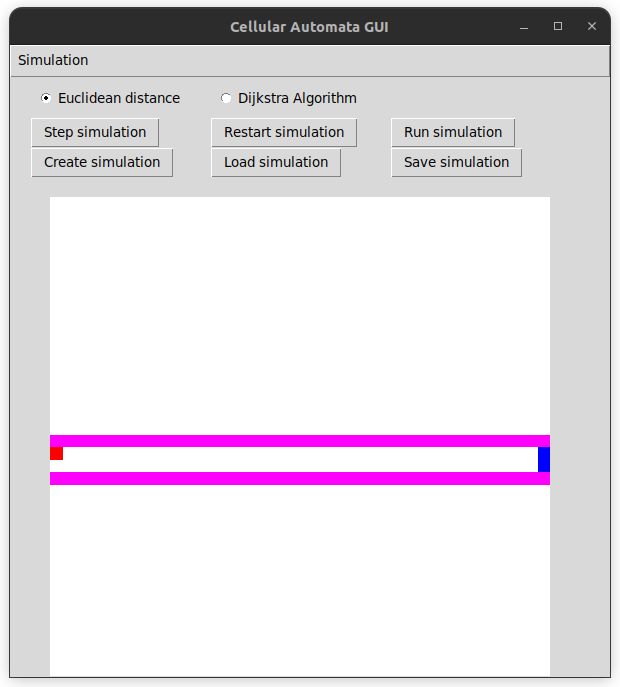
\includegraphics[width=\textwidth]{images/1-task1_initial.png}
    \caption{Automaton simulation}
    \label{fig: rimea_1a}
 \end{subfigure}
 \begin{subfigure}[b]{0.4\textwidth}
      \centering
     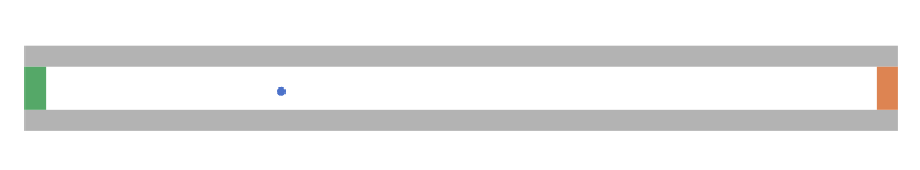
\includegraphics[width=\textwidth]{images/RIMEA1_2.png}
     \caption{Vadere simulation}
     \label{fig: rimea_1b}
 \end{subfigure}
 \caption{RiMEA scenario 1}
 \label{fig: rimea_1}
\end{figure}

\textbf{RiMEA scenario 6 (movement around a corner):}\\
Of course, the Vadere software makes it easier to recreate scenarios. The pedestrians get spawned randomly throughout the source which can simply be drawn out as a rectangle or another desired shape. The simulation for the RiMEA scenario 6 also differs: In our automaton, the pedestrians moved close to the border to take the shortest path to the target at the end of the corridor. The pedestrians in the OSM on the other side space out evenly, even if the path is a little longer that way. 

\begin{figure}[H]
 \centering
 \begin{subfigure}[b]{0.3\textwidth}
     \centering
     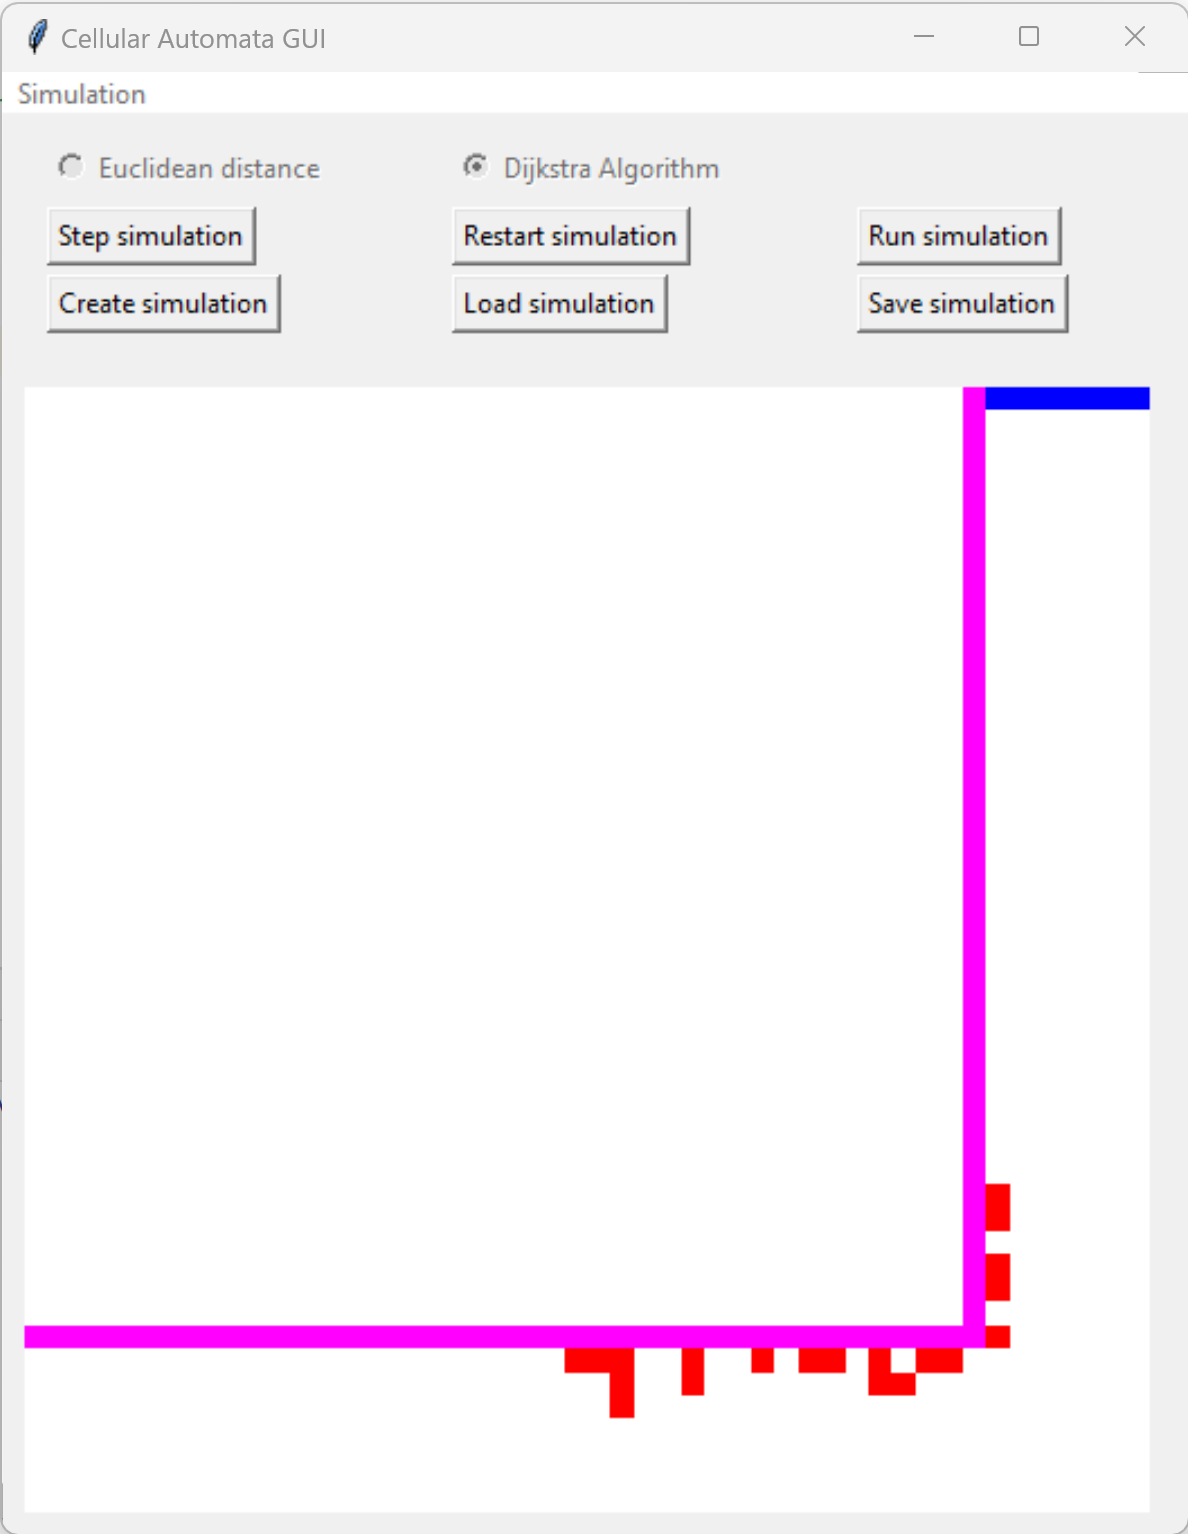
\includegraphics[width=\textwidth]{images/1-rimea6b.png}
    \caption{Automaton simulation}
    \label{fig: rimea_6a}
 \end{subfigure}
 \begin{subfigure}[b]{0.3\textwidth}
      \centering
     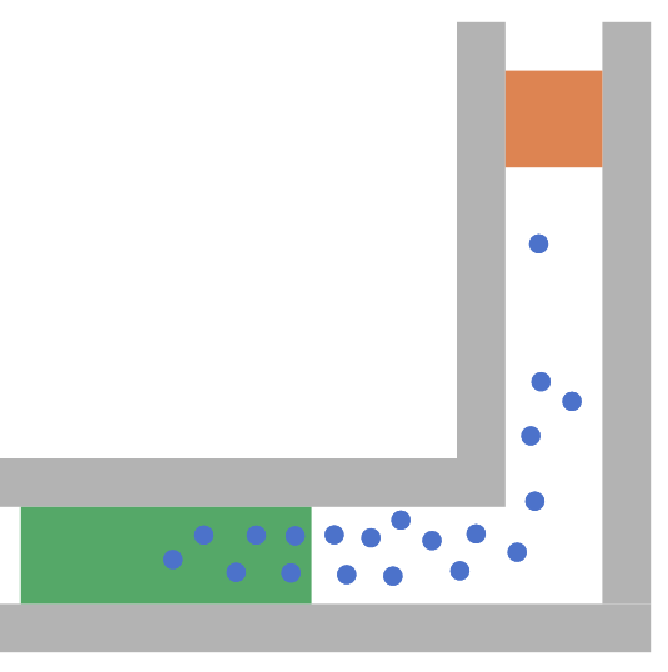
\includegraphics[width=\textwidth]{images/RIMEA6_2.png}
     \caption{Vadere simulation}
     \label{fig: rimea_6b}
 \end{subfigure}
 \caption{RiMEA scenario 6}
\label{fig: rimea_6}
\end{figure}



\textbf{Chicken Test:}\\
In our automaton, we can only see the current state of the simulation, whereas in Vadere we have the option to display trajectories which allow us to see the exact path the pedestrian took to reach the target. 

\begin{figure}[H]
 \centering
 \begin{subfigure}[b]{0.32\textwidth}
     \centering
     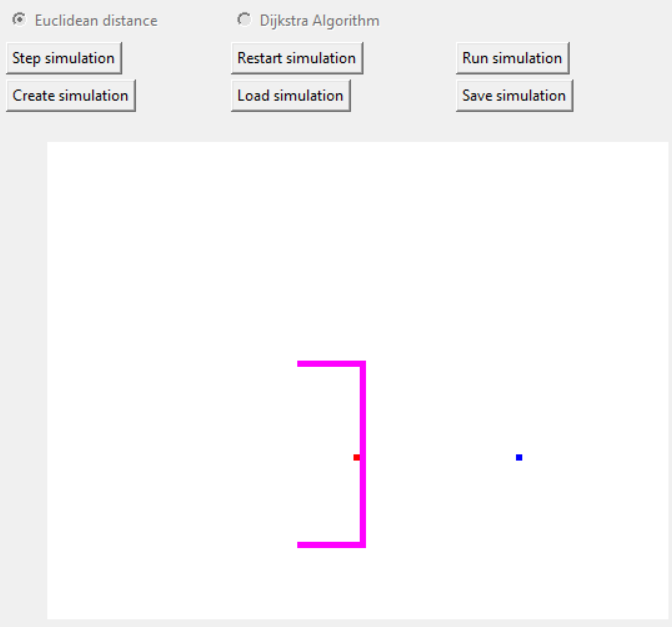
\includegraphics[width=\textwidth]{images/1-task4_chicken_first_contact.png}
    \caption{Automaton simulation}
    \label{fig: chicken-automaton}
 \end{subfigure}
 \begin{subfigure}[b]{0.3\textwidth}
      \centering
     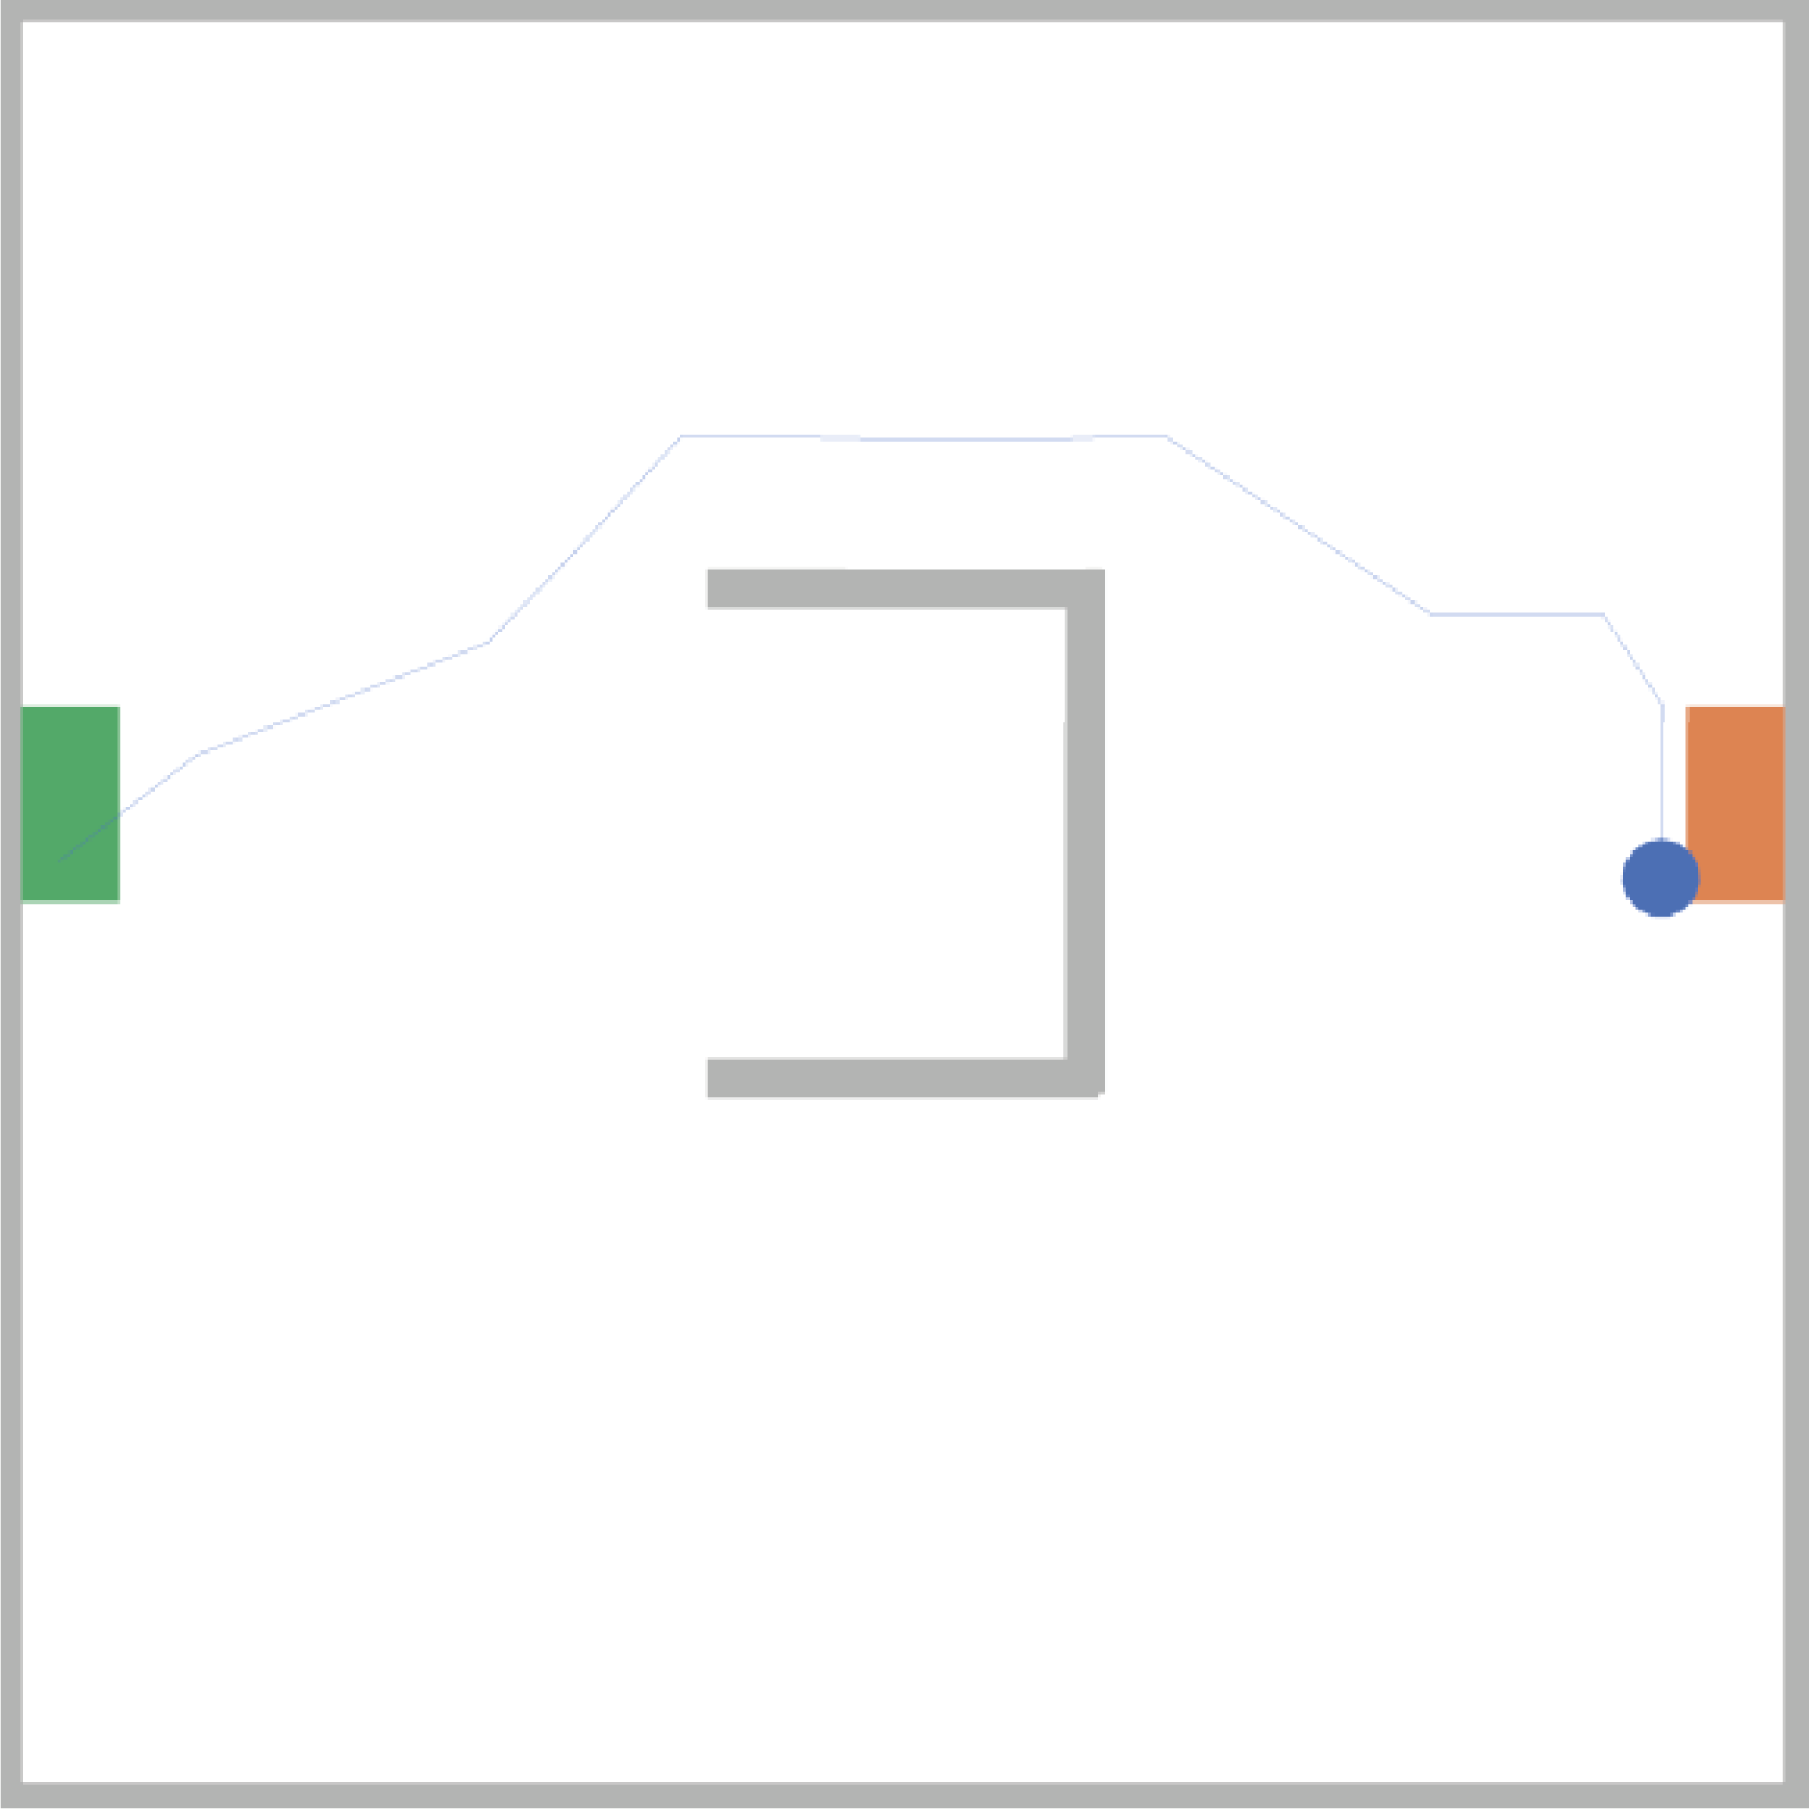
\includegraphics[width=\textwidth]{images/2-osm-chicken.png}
     \caption{Vadere simulation}
     \label{fig: chicken-vadere}
 \end{subfigure}
 \caption{Chicken Test}
\label{fig: chicken-task1}
\end{figure}